\documentclass{article}
\usepackage{eecstex}
\usepackage{pgfplots, pgfplotstable}
\usepackage{csvsimple}
\usepackage{mhchem}

\DeclareSIUnit\parsec{pc}
\DeclareSIUnit\year{yr}

\title{ASTRO 7A PS 10}
\author{Bryan Ngo}
\date{2020-11-28}

\begin{document}

\maketitle

\section{The Helix Nebula}

\begin{enumerate}
    \item A planetary nebula is the remains of a dead star after ejecting its outer shell.
    \item Note that \(\theta = \ang{;16;} = \SI{4.6}{\milli\radian}\) and \(d = \SI{213}{\parsec}\).
    Then, \(r = d \theta = \SI{0.99}{\parsec}\).
    \item \(t = \frac{d}{2v} = \SI{7.6e+11}{\second} = \SI{2.4e+4}{\year}\).
\end{enumerate}

\section{Evolution on the Main Sequence}

\subsection{}

The energy output of the star during the main sequence can be described as
\begin{equation}
    E = 0.1 \cdot 0.007 \cdot m c^2
\end{equation}
where \(m\) is the stellar mass and \(c\) is the speed of light.
\begin{center}
    \begin{tabular}{||l|l||}
        \hline
        \textbf{Mass} [\(M_\odot\)] & \textbf{Energy} [\si{\joule}]
        \csvreader[head to column names]{q2.csv}{}
        {\\ \mass & \energy}
        \\ \hline
    \end{tabular}
\end{center}

\subsection{}

\begin{center}
    \begin{tabular}{||l|l||}
        \hline
        \textbf{Mass} [\(M_\odot\)] & \textbf{Luminosity} [\(L_\odot\)]
        \csvreader[head to column names]{q2.csv}{}
        {\\ \mass & \luminosity}
        \\ \hline
    \end{tabular}
\end{center}

\subsection{}

\begin{center}
    \begin{tikzpicture}
        \begin{axis}[
            title=Logarithm of Mass vs. Logarithm of Luminosity,
            xlabel = {\(\log\left(\frac{M}{M_\odot}\right)\)},
            ylabel = {\(\log\left(\frac{L}{L_\odot}\right)\)},
        ]
        \addplot table[
            only marks,
            x=log-m, y=log-lum,
            col sep=comma,
        ] {q2.csv};
        \end{axis}
    \end{tikzpicture}
\end{center}
Thus, we have
\begin{equation}
    \log\left(\frac{L}{L_\odot}\right) \propto \log\left(\frac{M}{M_\odot}\right)
\end{equation}

\newpage
\section{Isochrones}

\subsection{}

At an age of \SI{100}{\mega\year}, about mass \(5 M_\odot\) or less stars remain, and at \SI{5}{\giga\year}, about mass \(1.25 M_\odot\) or less, giving us an HR diagram
\begin{center}
    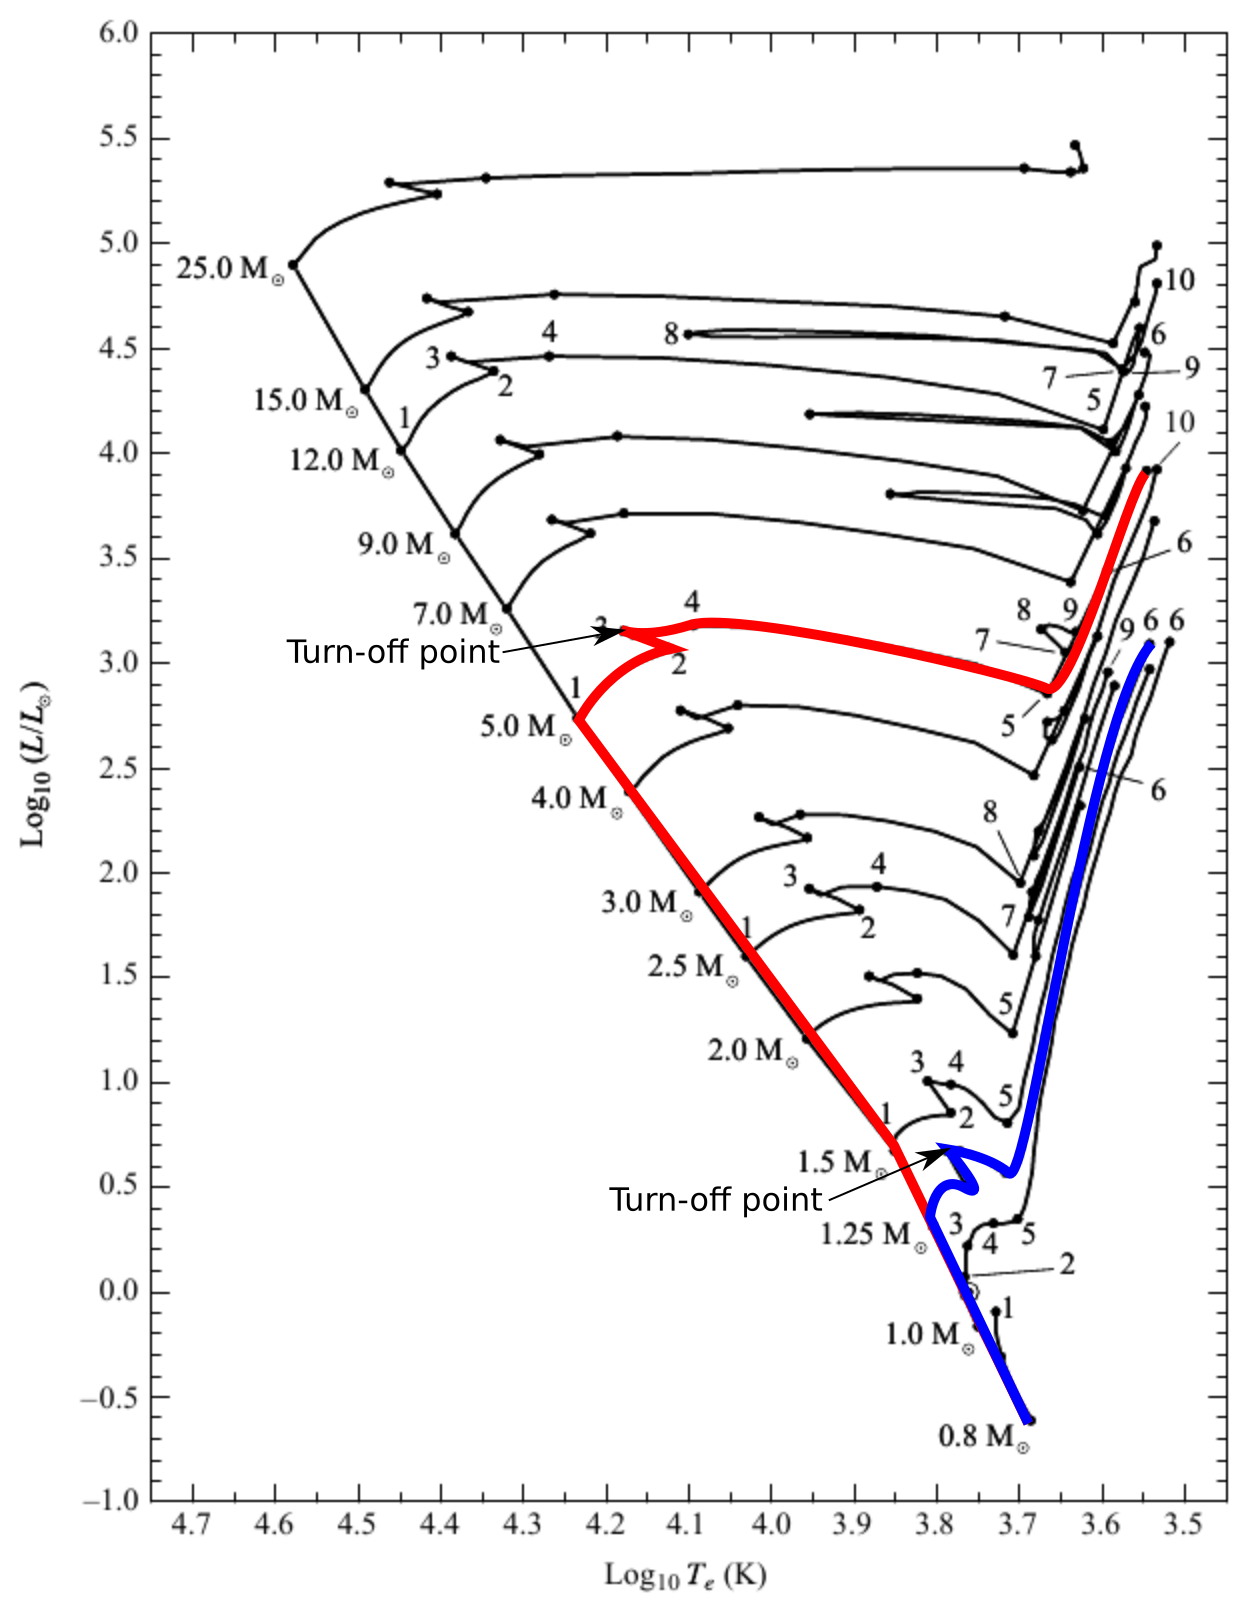
\includegraphics[width=0.5\textwidth]{q3a.png}
\end{center}

\subsection{}

\begin{equation}
    d = \SI{10}{\kilo\parsec}
\end{equation}
Observe that the turnoff point occurs at around \(m = 19\).
Converting to absolute magnitude using the distance modulus,
\begin{equation}
    M = m - 5 \log\left(\frac{d}{\SI{10}{\parsec}}\right) = 4
\end{equation}
Meaning that
\begin{equation}
    \log\left(\frac{L}{L_\odot}\right) = \frac{M_\odot - M}{2.5} = \num{0.332}
\end{equation}
Referring to Figure 13.1, this lands it at point 3 of a \(1 M_\odot\) cluster, or approximately \SI{4.91}{\giga\year}.

\subsection{}

\begin{enumerate}
    \item An interstellar cloud can absorb light and reemit redder light from a stellar cluster, which would make it appear dimmer and redder than it actually is; this is interstellar reddening.
    \item An interstellar cloud can also reflect bluer light from a stellar cluster by excitation of the dust grains, changing the received spectrum.
\end{enumerate}

\section{Horizontal Branch Lifetime}

\begin{align}
    M &= M_\odot \\
    \ce{^{4}_{2}He} &= \SI{4.0026}{\atomicmassunit} \\
    \ce{^{12}_{6}C} &= \SI{12.0000}{\atomicmassunit}
\end{align}

\begin{enumerate}
    \item The total mass lost in the triple alpha process is \(3 * \SI{4.0026}{\atomicmassunit} - \SI{12}{\atomicmassunit} = \SI{0.0078}{\atomicmassunit} = \SI{1.3e-29}{\kilogram}\), which by mass-energy equivalence is equal to \(\SI{1.2e-12}{\joule}\).
    \item The efficiency of the triple alpha process is \(\frac{\Delta m}{m} = \num{6.5e-4}\).
    Thus, \(E = (\num{6.5e-4}) \cdot 0.1 M_\odot c^2 = \SI{1.2e+43}{\joule}\).
    \item The luminosity of our star is \(L = L_\odot 10^{\frac{M_\odot - M}{5}} = \SI{3.828e+28}{\watt}\).
    Then, \(t = \frac{E}{L} = \SI{3.05e+15}{\second} = \SI{9.7e+6}{\year}\).
    This is about \num{1000} times smaller than the length of the main sequence of a \(1 M_\odot\) star.
\end{enumerate}

\section{SN 1987A}

\begin{align}
    \ce{^{56}_{27}Co} &= \SI{3.72}{\mega\electronvolt} \\
    \tau &= \SI{77.7}{\day} = \SI{6.7e+6}{\second} \\
    n &= \SI{1.3e+14}{\per\meter\squared} \\
    e_\nu &= \SI{4.2}{\mega\electronvolt} \\
    R &= \SI{50}{\kilo\parsec} \\
    M &= 1.4 M_\odot \\
    R_\star &= \SI{10}{\kilo\meter} 
\end{align}

\subsection{}

Using the formula for half-life
\begin{equation}
    N = N_0 e^{-\frac{\ln(2)}{\tau} t} \implies \frac{dN}{dt} = -\frac{\ln(2)}{\tau} N_0 e^{-\frac{\ln(2)}{\tau} t}
\end{equation}
the number of atoms in \(0.075 M_\odot\) of cobalt-56 is
\begin{equation}
    N_0 = 0.075 (\SI{2e+33}{\gram}) \cdot \frac{\SI{1}{\mole}}{\SI{56}{\gram}} \cdot N_A = \num{1.6e+54}
\end{equation}
Then,
\begin{align}
    L(0) &= (\SI{3.72}{\mega\electronvolt}) \left.\frac{dN}{dt}\right|_{t = 0} = \SI{-6.19e+53}{\electronvolt\per\second} = \SI{-9.9e+34}{\watt} \\
    L(500) &= (\SI{3.72}{\mega\electronvolt}) \left.\frac{dN}{dt}\right|_{t = 500} = \SI{-7.1e+51}{\electronvolt\per\second} = \SI{-1.15e+33}{\watt}
\end{align}

\subsection{}

We can express the flux as
\begin{equation}
    E = 4 \pi R^2 e_\nu n = \SI{1.63e+64}{\electronvolt} = \SI{2.62e+45}{\joule}
\end{equation}

\subsection{}

The binding energy can be defined as
\begin{equation}
    U = -\frac{3}{5} \frac{GM^2}{R_\star} = \SI{-3.14e+46}{\joule}
\end{equation}
So the neutrino energy is about \num{8.3}\% of the gravitational binding energy.

\end{document}
